\documentclass[aspectratio=169]{beamer}
\usetheme{Madrid}
\usecolortheme{dolphin}
\usepackage{booktabs}
\usepackage{graphicx}
\usepackage{hyperref}
\usepackage{listings}
\usepackage{xcolor}
\usepackage{tikz}
\usetikzlibrary{shapes,arrows,positioning}

% Custom colors
\definecolor{esblue}{RGB}{79,70,229}
\definecolor{esviolet}{RGB}{124,58,237}
\definecolor{esgray}{RGB}{17,24,39}

\setbeamercolor{palette primary}{bg=esblue,fg=white}
\setbeamercolor{palette secondary}{bg=esviolet,fg=white}
\setbeamercolor{title}{fg=esblue}
\setbeamercolor{frametitle}{bg=esblue,fg=white}
\setbeamercolor{structure}{fg=esblue}

% Title Information — fill in your details
\title[EngageSphere]{\textbf{EngageSphere}}
\subtitle{AI-Powered Multi-Platform Customer Engagement System}
\author{[Your Name(s)]}
\institute{[Your College / University]}
\date{[Semester / Year]}

% ============================================================
\begin{document}
% ============================================================

% --- Title Slide ---
\begin{frame}
  \titlepage
\end{frame}

% --- Outline ---
\begin{frame}{Outline}
  \tableofcontents
\end{frame}

% ============================================================
\section{Methodology}
% ============================================================

\begin{frame}{Problem Statement}
  \begin{block}{The Challenge}
    Small and medium business owners receive customer feedback scattered across
    \textbf{Google Maps, Facebook, Instagram, and Twitter}.
  \end{block}
  \vspace{0.4cm}
  \begin{itemize}
    \item Responding manually is \textbf{time-consuming} and \textbf{inconsistent}
    \item Delayed responses hurt \textbf{customer satisfaction} and \textbf{brand reputation}
    \item No single tool aggregates, replies, and suggests improvements across all platforms
  \end{itemize}
\end{frame}

\begin{frame}{Proposed Solution}
  \textbf{EngageSphere} is an AI-powered, multi-platform customer engagement system that:
  \vspace{0.3cm}
  \begin{enumerate}
    \item \textbf{Ingests} customer reviews and comments from all platforms
    \item \textbf{Classifies} sentiment and intent using NLP
    \item \textbf{Generates} brand-appropriate AI replies grounded in business facts (RAG)
    \item \textbf{Surfaces} actionable improvement suggestions from aggregated feedback
    \item \textbf{Posts} approved replies back to the platform — with human review
  \end{enumerate}
\end{frame}

\begin{frame}{Development Methodology}
  \textbf{Agile Phased Development} — 9 independent phases, each verified before next:
  \vspace{0.2cm}
  \begin{table}
    \centering
    \small
    \begin{tabular}{@{}clc@{}}
      \toprule
      \textbf{Phase} & \textbf{Description} & \textbf{Status} \\
      \midrule
      1 & Project scaffolding + database schema & \textcolor{green!60!black}{Complete} \\
      2 & Mock data connectors (Google Maps, Twitter) & \textcolor{green!60!black}{Complete} \\
      3 & Live connectors (Facebook, Instagram) & \textcolor{green!60!black}{Complete} \\
      4 & Sentiment + intent classification & \textcolor{green!60!black}{Complete} \\
      5+6 & AI reply generation + approval workflow & \textcolor{green!60!black}{Complete} \\
      7 & Suggestion Agent (RAG-powered) & \textcolor{green!60!black}{Complete} \\
      8 & Unified dashboard frontend & \textcolor{green!60!black}{Complete} \\
      9 & Polish, testing, demo preparation & \textcolor{green!60!black}{Complete} \\
      \bottomrule
    \end{tabular}
  \end{table}
\end{frame}

% ============================================================
\section{Algorithm / Block Diagram}
% ============================================================

\begin{frame}{System Architecture}
  \begin{center}
  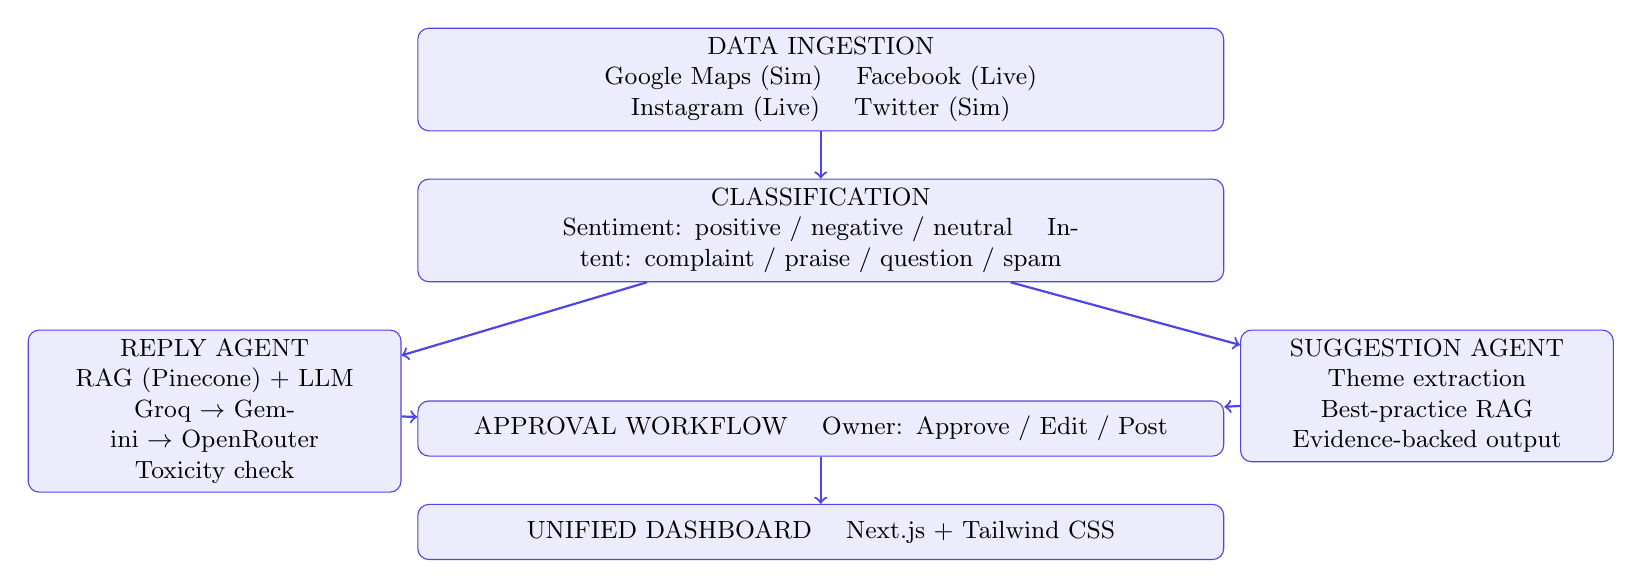
\begin{tikzpicture}[
    node distance=0.6cm,
    box/.style={rectangle, rounded corners, draw=esblue, fill=esblue!10,
                text width=3cm, align=center, minimum height=0.7cm, font=\small},
    arrow/.style={->, thick, color=esblue}
  ]
    \node[box, text width=10cm] (ingest)
      {DATA INGESTION\\
       \small Google Maps (Sim) \quad Facebook (Live) \quad Instagram (Live) \quad Twitter (Sim)};

    \node[box, text width=10cm, below=of ingest] (classify)
      {CLASSIFICATION\\
       \small Sentiment: positive / negative / neutral \quad
       Intent: complaint / praise / question / spam};

    \node[box, text width=4.5cm, below left=0.6cm and 0.2cm of classify] (reply)
      {REPLY AGENT\\
       \small RAG (Pinecone) + LLM\\
       Groq $\to$ Gemini $\to$ OpenRouter\\
       Toxicity check};

    \node[box, text width=4.5cm, below right=0.6cm and 0.2cm of classify] (suggest)
      {SUGGESTION AGENT\\
       \small Theme extraction\\
       Best-practice RAG\\
       Evidence-backed output};

    \node[box, text width=10cm, below=1.5cm of classify] (approval)
      {APPROVAL WORKFLOW \quad Owner: Approve / Edit / Post};

    \node[box, text width=10cm, below=of approval] (dashboard)
      {UNIFIED DASHBOARD \quad Next.js + Tailwind CSS};

    \draw[arrow] (ingest) -- (classify);
    \draw[arrow] (classify) -- (reply);
    \draw[arrow] (classify) -- (suggest);
    \draw[arrow] (reply) -- (approval);
    \draw[arrow] (suggest) -- (approval);
    \draw[arrow] (approval) -- (dashboard);
  \end{tikzpicture}
  \end{center}
\end{frame}

\begin{frame}{LLM Failover Chain \& Toxicity Gate}
  \begin{block}{LLM Failover Chain}
    \centering
    \texttt{Request $\rightarrow$ Groq (Llama 3) $\xrightarrow{\text{fail}}$ Gemini $\xrightarrow{\text{fail}}$ OpenRouter $\xrightarrow{\text{fail}}$ Error}
  \end{block}
  \vspace{0.4cm}
  \begin{block}{Toxicity Gate (every generated reply)}
    \centering
    \texttt{Generated Reply $\rightarrow$ toxic-bert classifier}\\
    \vspace{0.2cm}
    \begin{itemize}
      \item Score $\geq$ 0.7 $\Rightarrow$ \textcolor{red}{Flag for manual review}
      \item Score $<$ 0.7 $\Rightarrow$ \textcolor{green!60!black}{Enter approval queue}
    \end{itemize}
  \end{block}
  \vspace{0.2cm}
  \small Note: Spam items (detected by intent classifier) are excluded from reply queue entirely.
\end{frame}

% ============================================================
\section{Implementation}
% ============================================================

\begin{frame}{Tech Stack}
  \begin{columns}
    \column{0.5\textwidth}
    \begin{table}
      \small
      \begin{tabular}{@{}ll@{}}
        \toprule
        \textbf{Layer} & \textbf{Technology} \\
        \midrule
        Backend & FastAPI (Python, async) \\
        Frontend & Next.js 15 + Tailwind \\
        Database & Supabase (PostgreSQL) \\
        Auth & Supabase Auth (JWT) \\
        LLM & Groq $\to$ Gemini $\to$ OpenRouter \\
        \bottomrule
      \end{tabular}
    \end{table}

    \column{0.5\textwidth}
    \begin{table}
      \small
      \begin{tabular}{@{}ll@{}}
        \toprule
        \textbf{Layer} & \textbf{Technology} \\
        \midrule
        Toxicity & toxic-bert (local) \\
        Vector Store & Pinecone (RAG) \\
        Embeddings & sentence-transformers \\
        Live APIs & Meta Graph API \\
        Simulated & Mock JSON datasets \\
        \bottomrule
      \end{tabular}
    \end{table}
  \end{columns}
\end{frame}

\begin{frame}{Key Implementation Features}
  \begin{itemize}
    \item \textbf{Multi-tenant architecture} — each business has isolated data and platform connections
    \item \textbf{Human-in-the-loop} — no reply ever auto-posted without owner approval
    \item \textbf{RAG grounding} — replies use actual business facts from Pinecone, preventing hallucination
    \item \textbf{Deduplication} — same comment never ingested twice (platform + external\_id + business\_id)
    \item \textbf{Connector isolation} — one connector failure never crashes the pipeline
    \item \textbf{OAuth flow} — business owners connect social accounts with one click (no token copying)
  \end{itemize}
\end{frame}

\begin{frame}{Database Schema}
  \textbf{5 core tables in PostgreSQL (Supabase):}
  \vspace{0.3cm}
  \begin{table}
    \small
    \begin{tabular}{@{}ll@{}}
      \toprule
      \textbf{Table} & \textbf{Purpose} \\
      \midrule
      \texttt{businesses} & Business accounts (name, user\_id, email) \\
      \texttt{platform\_connections} & Per-business OAuth tokens per platform \\
      \texttt{feedback\_items} & All ingested comments/reviews (sentiment, intent) \\
      \texttt{replies} & AI-generated replies with approval status \\
      \texttt{suggestions} & AI-generated improvement recommendations \\
      \bottomrule
    \end{tabular}
  \end{table}
  \vspace{0.3cm}
  All tables scoped by \texttt{business\_id} — full multi-tenant isolation.
\end{frame}

% ============================================================
\section{Demonstration}
% ============================================================

\begin{frame}{Demo Flow}
  \begin{enumerate}
    \item \textbf{Sign Up / Login} — Email + password via Supabase Auth
    \item \textbf{Fetch Comments} — Pulls from all 4 platforms (30 items from mock + live)
    \begin{itemize}
      \item Google Maps: 15 reviews (ratings 1--5, mix of sentiment)
      \item Twitter/X: 15 mentions (including spam for testing)
    \end{itemize}
    \item \textbf{Filter} — By platform (Google Maps / Facebook / Instagram / Twitter)
    \item \textbf{Filter} — By sentiment (Positive / Negative / Neutral)
    \item \textbf{Generate Replies} — AI creates brand-appropriate reply per comment
    \item \textbf{Approve + Post} — Owner approves $\rightarrow$ reply posted live
    \item \textbf{Suggestions} — Re-generate $\rightarrow$ 3--5 evidence-backed recommendations
  \end{enumerate}
\end{frame}

\begin{frame}{Demo Highlights}
  \begin{block}{Sentiment Breakdown}
    Live chart shows percentage split: Positive / Negative / Neutral across all platforms
  \end{block}
  \vspace{0.3cm}
  \begin{block}{AI Reply Example}
    \small\textit{Customer: ``Waited 30 minutes, no apology from staff.''}\\
    \textit{AI Reply: ``We're truly sorry for the wait you experienced — that's not the standard of service we aim to provide. We're reviewing our peak-hour processes and will ensure the team acknowledges delays promptly. We hope to welcome you back and make it right.''}
  \end{block}
  \vspace{0.2cm}
  \begin{itemize}
    \small
    \item Grounded in business facts (hours, policies) — no hallucination
    \item Spam auto-excluded, toxicity auto-flagged
  \end{itemize}
\end{frame}

% ============================================================
\section{IPR Status}
% ============================================================

\begin{frame}{Intellectual Property Rights (IPR) Status}
  \begin{block}{Current Status: Not Filed}
    The project uses open-source components under permissive licenses (MIT, Apache 2.0).
  \end{block}
  \vspace{0.3cm}
  \textbf{Potential IPR Opportunities:}
  \begin{itemize}
    \item Multi-platform aggregation + RAG-grounded reply generation pipeline
    \item Theme-based Suggestion Agent with evidence-quote extraction methodology
    \item Eligible for \textbf{provisional patent application} as a business method patent
  \end{itemize}
  \vspace{0.3cm}
  \textbf{Open-source components used:}
  \begin{itemize}
    \small
    \item FastAPI (MIT), Next.js (MIT), Supabase (Apache 2.0)
    \item Hugging Face Transformers (Apache 2.0), sentence-transformers (Apache 2.0)
    \item unitary/toxic-bert (MIT)
  \end{itemize}
\end{frame}

% ============================================================
\section{Hackathons / Competitions}
% ============================================================

\begin{frame}{Hackathons \& Project Competitions}
  \begin{block}{Participation Status}
    \textbf{Currently planning participation} in the following events:
  \end{block}
  \vspace{0.3cm}
  \begin{table}
    \small
    \begin{tabular}{@{}llll@{}}
      \toprule
      \textbf{Event} & \textbf{Type} & \textbf{Venue} & \textbf{Date} \\
      \midrule
      Smart India Hackathon (SIH) & National & TBD & 2026 \\
      HackWithInfy & Industry & TBD & 2026 \\
      Hack This Fall & Open (Online) & Online & 2026 \\
      IEEE Student Project Expo & Technical & TBD & 2026 \\
      \bottomrule
    \end{tabular}
  \end{table}
  \vspace{0.3cm}
  \small \textit{Update this slide with actual events participated in or registered for.}
\end{frame}

% ============================================================
\section{Conclusion}
% ============================================================

\begin{frame}{Conclusion}
  \textbf{EngageSphere successfully demonstrates:}
  \vspace{0.2cm}
  \begin{enumerate}
    \item \textbf{Multi-platform ingestion} — 4 platforms through a unified pipeline
    \item \textbf{Automated NLP classification} — sentiment, intent, and spam detection
    \item \textbf{RAG-grounded AI reply generation} — factually accurate, toxicity-checked
    \item \textbf{Evidence-backed suggestions} — actionable recommendations from feedback
    \item \textbf{Production-ready architecture} — multi-tenant, JWT-authenticated
  \end{enumerate}
\end{frame}

\begin{frame}{Impact \& Future Scope}
  \begin{columns}
    \column{0.5\textwidth}
    \textbf{Impact:}
    \begin{itemize}
      \item Response time: hours $\rightarrow$ seconds
      \item Consistent brand voice across all platforms
      \item Surfaces recurring issues automatically
      \item Scalable to any number of businesses
    \end{itemize}

    \column{0.5\textwidth}
    \textbf{Future Scope:}
    \begin{itemize}
      \item WhatsApp Business API integration
      \item Automated reply scheduling
      \item Sentiment trend analytics over time
      \item Multi-language reply generation
      \item Mobile app for on-the-go approval
    \end{itemize}
  \end{columns}
\end{frame}

% ============================================================
\section{References}
% ============================================================

\begin{frame}{References}
  \footnotesize
  \begin{enumerate}
    \item Brown, T. et al. (2020). \textit{Language Models are Few-Shot Learners}. NeurIPS.
    \item Lewis, P. et al. (2020). \textit{Retrieval-Augmented Generation for Knowledge-Intensive NLP Tasks}. NeurIPS.
    \item Liu, Y. et al. (2019). \textit{RoBERTa: A Robustly Optimized BERT Pretraining Approach}. arXiv:1907.11692.
    \item Houlsby, N. et al. (2019). \textit{Parameter-Efficient Transfer Learning for NLP}. ICML.
    \item Meta Platforms Inc. (2024). \textit{Meta Graph API Documentation}. \url{https://developers.facebook.com/docs/graph-api/}
    \item Supabase Inc. (2024). \textit{Supabase Documentation}. \url{https://supabase.com/docs}
    \item Pinecone Systems Inc. (2024). \textit{Pinecone Vector Database Documentation}. \url{https://docs.pinecone.io}
    \item Groq Inc. (2024). \textit{Groq API Documentation}. \url{https://console.groq.com/docs}
    \item Hugging Face (2024). \textit{twitter-roberta-base-sentiment-latest}. \url{https://huggingface.co/cardiffnlp}
    \item Reimers, N. \& Gurevych, I. (2019). \textit{Sentence-BERT: Sentence Embeddings using Siamese BERT-Networks}. EMNLP.
  \end{enumerate}
\end{frame}

% --- Thank You ---
\begin{frame}
  \begin{center}
    \vspace{1cm}
    {\Huge \textbf{Thank You}}\\
    \vspace{0.8cm}
    {\large Questions?}\\
    \vspace{1cm}
    \textcolor{esblue}{\textbf{EngageSphere}}\\
    \small AI-Powered Multi-Platform Customer Engagement System
  \end{center}
\end{frame}

\end{document}
